% 2006 安徽文科 Q9；函数与标注按固定来源重绘。
\begin{tikzpicture}[x=1.45cm,y=0.95cm,line cap=round,line join=round,>=stealth,font=\small]
  \draw[->] (-0.9,0) -- (3.4,0) node[right] {$x$};
  \draw[->] (0,-1.5) -- (0,1.65) node[above] {$y$};
  \draw[thick,domain=-0.8:3.0,samples=140] plot (\x,{sin(deg(2*\x+pi/3))});
  \draw[dashed] ({7*pi/12},0) -- ({7*pi/12},-1) -- (0,-1);
  \node[below right] at (0,0) {$O$};
  \node[left] at (0,1) {$1$};
  \node[left] at (0,-1) {$-1$};
  \node[above] at ({7*pi/12},0) {$\dfrac{7\pi}{12}$};
\end{tikzpicture}
